\documentclass[11pt,a4paper]{article}

\usepackage{graphicx}
\usepackage{color}
\usepackage{amsmath}
\usepackage{amssymb}
\usepackage{listings}
\usepackage{hyperref}

\lstset{language=c++}
\lstset{basicstyle=\tiny}
\lstset{backgroundcolor=\color{white}}
\lstset{frame=single}
\lstset{stringstyle=\ttfamily}
\lstset{keywordstyle=\color{red}\bfseries}
\lstset{commentstyle=\itshape\color{blue}}
\lstset{showspaces=false}
\lstset{showstringspaces=false}
\lstset{showtabs=false}
\lstset{breaklines}

\title{Comparison of Linear Algebra Metholodigies in Solving a Second Order Differential Equation}
\author{John Bower}
\date{February 12 2016}

\begin{document}
\maketitle

\begin{abstract}

	In this project I solve a linear second order differential equation using three different linear algebra methodologies in order to compare their computational speed, accuracy, and stability. Included herein are an LU decomposition, a general tridiagonal matrix solver, and a tridiagonal solver specific to our form. I find that while all three have a similar trend in accuracy, the speed and stabilities differ. The solver specific to the presented case is the fastest and most stable, whereas the general tridiagonal solver is approximately one-third slower and loses stability sooner. LU decomposition lags behind with vast increases in computation time with no gain in accuracy.

\end{abstract}

\begin{itemize}
\item All source files and benchmark calculations can be found at \url{https://github.com/johnbower2012/CPMSU_work/tree/master/project1}.
\item A list of all code files can be found at the end of this document.
\end{itemize}

\section{Introduction}

Many important equations in Physics can be reduced to a linear second order differential equation of the form
\[
\frac{d^2y}{dx^2} + k^2(x)y = f(x),
\]
which is called $inhomogenous$ if $f \neq 0$ and $homogenous$ if $f = 0$. 
A traditional example is Poisson's equation from electromagnetism, wherein is found an electrostatic potential $\Phi$ generated by a charge distribution $\rho (\bf{r})$. In three dimensions this can be written as
\[
\nabla^2\Phi = -4\pi\rho(\bf{r}).
\]
Provided that both $\Phi$ and $\rho(\bf{r})$ are spherically symmetric, Poisson's equation simplifies to a single dimension, denoted here as $r$,
\[
\frac{1}{r^2}\frac{d}{dr}(r^2\frac{d\Phi}{dr}) = -4\pi\rho(r)
\]
Manipulating the equation, we see that if we replace $\Phi(r)$ by $\frac{\phi(r)}{r}$, we arrive at
\[
\frac{d^2\phi}{dr^2} = -4\pi r\rho(r)
\]
Rewriting $\phi\rightarrow u$ and $r\rightarrow x$ allows us to write
\[
\frac{d^2u}{dx^2} = -4\pi x \rho (x)
\]
From here, we can finally recognize $4\pi x \rho(x)$ as the inhomogenous term $f(x)$, resulting in our final equation of
\[
-u''(x) = f(x).
\]
Our aim in this project is to solve this problem numerically by discretizing the domain and implementing methods from linear algebra. We will begin by solving the general LU decompisition problem to test for numerical accuracy, speed, and stability. From there we will refine our approach and show how this problem may be solved much more simply, first by a general tridiagonal solver and then by a tridiagonal solver tailored to our particular case, allowing for a great reduction in computation time and an increase in stability.

\section{Theory}

The specific case which will be detailed in this project will use Dirichlet boundary conditions,
\begin{equation}
-u''(x)=f(x), \hspace{0.5 cm} x\in(0,1), \hspace{0.5 cm} u(0) = u(1) = 0.
\end{equation}
We begin by discretizing the domain into $n$ grid points, excluding end points, with step spacing $h = 1/(n+1)$ such that $x_0 = 0, \dots , x_i = ih, \dots x_{n+1} = 1$. Approximating $u(x)$ with the discretized function $v(x_i)$, so that $u(x_i) \approx v(x_i) = v_i$, we use the following approximation
\begin{equation}
-u''(x) = -\frac{v_{i+1} - 2v_i + v_{i-1}}{h^2} = f(x_i) = f_i.
\end{equation}
Multiplying both sides by $h^2$ and distributing through the negative sign, we arrive at the evocative form
\begin{equation}
-v_{i+1} + 2v_i - v_{i-1} = h^2 f_i \equiv f_i, 
\end{equation}
where we have simply absorbed the $h^2$ into the $f_i$ since we have not yet defined $f$ itself. Defining the constants next to each $v_j$ as $a_{ij}$,
\begin{equation}
a_{i(i+1)} v_{i+1} + a_{ii} v_i + a_{i(i-1)} v_{i-1} = f_i.
\end{equation}
We see that this is nothing more than an equivalent of matrix multiplication,
\begin{equation}
\sum\limits_{j=1}^n a_{ij} v_{j} = f_i,
\end{equation}
where each $a_{ij}$ is defined by $a_{i=j} = 2, \hspace{0.2 cm} a_{|i-j|=1} = 1, \hspace{0.2 cm} a_{|i-j|>1} = 0$, so that we arrive at $\bf{A}*\hat{v} = \hat{f}$, or
\begin{equation}
\left(\begin{array}{cccccc}
			    2 & -1 & 0 & \dots & \dots & 0 \\
			    -1 & 2 & -1 & \dots & \dots & 0 \\
			    0 & -1 & 2 & -1 & 0 & \dots \\
			    \dots & \dots & \dots & \dots & \dots & \dots \\
			    \dots & \dots & 0 & -1 & 2 & -1 \\
                            \dots & \dots & \dots & 0 & -1 & 2 \end{array} \right)
			\left(\begin{array}{c}
			    v_1 \\
			    v_2 \\
			    \dots \\
			    \dots \\
			    \dots \\
			    v_n \end{array} \right)
	=\left(\begin{array}{c}
			    f_1 \\
			    f_2 \\
			    \dots \\
			    \dots \\
			    \dots \\
			    f_n \end{array} \right).
\end{equation}
Given an initial $f$, we are then able to solve the second order differential equation as a linear algebra problem wherein we find $\hat{v}$.

In this project we test the algorithms with $f(x) = 100e^{-10x}$. This is a simple example problem to test, where the analytical solution is known to be $u(x) = 1 - (1-e^{-10}) x - e^{-10x}$. This will be the solution with which we determine the accuracy of our final numerical results.


\section{Methodology}

In this section we discuss the implementation of the three algorithms designed to solve the differential equation presented in this project, by performing an LU decompisition, by solving a general tridiagonal matrix, and by recognizing the symmetries inherent to our selected approximation. My own code written for this task is included in my github repository, as seen at the beginning of the project, which also includes options for printing error and computation time to file. 

\subsection{LU Decomposition}

LU decompisition is an operation whereby one decomposes {\bf A} into a multiplication of two matrices, {\bf L}, a unit lower triangular matrix, and {\bf U}, an upper triangular matrix, as follows,
\begin{equation*}
\left(\begin{array}{cccc}
			a_{11} & a_{12} & \dots & a_{1n} \\
			a_{21} & a_{22} & \dots & \dots \\
			\dots & \dots & \dots & \dots \\
			a_{1n} & \dots & \dots & a_{nn} \end{array} \right)
	=\left(\begin{array}{cccc}
			1 & 0 & \dots & 0 \\
			l_{21} & 1 & \dots & 0 \\
			\dots & \dots & \dots & \dots \\
			l_{n1} & \dots & l_{nn-1} & 1 \end{array} \right)
		\left(\begin{array}{cccc}
			u_{11} & u_{12} & \dots & u_{1n} \\
			0 & u_{22} & \dots & u_{2n} \\
			\dots & \dots & \dots & \dots \\
			0 & \dots & 0 & u_{nn} \end{array} \right).
\end{equation*}
It should be noted that simple LU decomposition is not possible for all matrices, and that some pivoting may be required. Here we address the simpler case of no pivoting.
Performing the basic matrix multiplication, we see that
\begin{align*}
a_{1j} &= u_{1j} \\
a_{i1} &= l_{i1}u_{11}, \hspace{0.5 cm} i>1 \\
a_{2j} &= u_{2j} + l_{21}u_{1j}, \hspace{0.5 cm} j>1 \\
a_{i2} &= l_{i2}u_{22} + l_{i1}u{12}, \hspace{0.5 cm} i>2 \\
&\vdots \\
a_{ij} &= \sum\limits_{k=1}^n l_{ik}u_{kj}
\end{align*}
Observing carefully, one sees that at each row there is only one unknown, with all previous unknowns found previously. Rearranging to solve for $u_{ij}$ and $l_{ij}$,
\begin{align*}
u_{1j} =& a_{1j} \\
l_{i1} =& \frac{a_{i1}}{u_{11}}, \hspace{0.5 cm} i>1 \\
u_{2j} =& a_{2j} - l_{21}u_{1j}, \hspace{0.5 cm} j>1 \\
l_{i2} =& \frac{a_{i2} - l_{i1}u_{12}}{u_{22}}, \hspace{0.5 cm} i>2 \\
&\vdots \\
\end{align*}
\begin{align}
u_{ij} =& a_{ij} - \sum\limits_{k=1}^{i-1} l_{ik}u_{kj}, \hspace{0.5 cm} u_{1j} \equiv a_{1j},\\
l_{ji} =& \frac{a_{ji} - \sum\limits_{k=1}^{i-1} l_{jk}u_{ki}}{u_{ii}}, \hspace{0.5 cm} l_{j1} \equiv \frac{a_{j1}}{u_{11}}
\end{align}
where the indices on the final $l_{ji}$ have been purposefully switched with respect to $u_{ij}$ in order represent the pattern observed in previous iterations.

With both {\bf L} and {\bf U} determined, we define a vector $\hat{y} = {\bf U}*\hat{v}$ such that ${\bf L}*\hat{y} = \hat{f}$. Given the unit lower triangular form of {\bf L}, solving for $\hat{y}$ becomes simple. Multiplying through we see $y_1 = f_1$, \hspace{0.1 cm} $l_{21}y_1 + y_2 = f_2$, \hspace{0.1 cm} \dots, \hspace{0.1 cm} $\sum\limits_{k=1}^n l_{nk}y_k = f_n$, and so solving for each $y_{i}$ we derive 
\begin{equation}
y_{i} = f_{i} - \sum\limits_{k=1}^{i-1} l_{ik}y_k, \hspace{0.5 cm} y_1 \equiv f_1.
\end{equation}

With $\hat{y}$, we then solve ${\bf U}*\hat{v} = \hat{y}$ for $\hat{v}$. Once more, multiplying through we see $u_{11}v_1 + \dots + u_{1n}v_n = y_1$, \hspace{0.2 cm} $u_{22}v_2 + \dots + u_{2n}v_n = y_1$, \hspace{0.1 cm} \dots \hspace{0.1 cm} $u_{nn}v_n = y_n$. Via back substitution, we arrive at our solution for $\hat{v}$,
\begin{equation}
v_i = \frac{y_i - \sum\limits_{k=1}^{i-1} u_{ik}v_k}{u_{ii}}, \hspace{0.5 cm} v_n \equiv \frac{y_n}{u_{nn}}.
\end{equation}

It should be observed that this process is very expensive; the leading term in the number of floating point operations from equations (6) through (10) runs as ~ $\frac{2}{3}n^3$. Care should be taken for large choices of n, as an increase by a magnitude of ten in $n$ results in a 1000 fold increase in computation time.

\subsection{General Tridiagonal}

In order to refine and reduce our performed computations, we recognize that the matrix {\bf A} is tridiagonal in form, that is that all elements $a_{ij}$, such that $|i-j|>1$, are zero. Rewriting
\begin{equation*}
{\bf A} = \left(\begin{array}{cccccc}
			b_1 & c_1 & 0 & \dots & \dots & 0 \\
			a_2 & b_2 & c_2 & 0 & \dots & 0 \\
			0 & a_3 & b_3 & c_3 & \dots & 0 \\
			\dots & \dots & \dots & \dots & \dots & \dots \\
			0 & \dots & 0 & a_{n-1} & b_{n-1} & c_{n-1} \\
			0 & \dots & \dots & 0 & a_n & b_n \end{array} \right),
\end{equation*}
we see {\bf A} can be represented properly by three arrays, denoted here as $\hat{a}$, $\hat{b}$, and $\hat{c}$ (note that we say $a_1 \equiv c_n \equiv$ 0). From here, we perform operations to form {\bf A} into an upper triangular matrix, as follows
\begin{equation*}
\left(\begin{array}{ccccc}
			b_1 & c_1 & 0 & \dots & 0 \\
			0 & b_2 - c_1\frac{a_2}{b_1} & c_2 & \dots & 0 \\
			\dots & \dots & \dots & \dots & \dots \\
			\dots & \dots & \dots & \dots & \dots \\
			0 & \dots & \dots & 0 & b_n - c_{n-1}\frac{a_n}{b_{n-1}} \end{array} \right)
		\left(\begin{array}{c}
			v_1 \\
			v_2 \\
			\dots \\
			\dots \\
			v_n \end{array} \right)
		=\left(\begin{array}{c}
			f_1 \\
			f_2 - f_1\frac{a_2}{b_1} \\
			\dots \\
			\dots \\
			f_n - f_{n-1}\frac{a_n}{b_{n-1}} \end{array} \right)
\end{equation*}
Denoting
\begin{equation}
\tilde{b_i} = b_i - c_{i-1}\frac{a_i}{b_{i-1}}, \hspace{0.5 cm} \tilde{b_1} \equiv b_1, \\
\end{equation}
and
\begin{equation}
\tilde{f_i} = f_i - f_{i-1}\frac{a_i}{b_{i-1}}, \hspace{0.5 cm} \tilde{f_1} \equiv f_1,
\end{equation}
 we are able to perform back substition to solve for $\hat{v}$,
\begin{equation}
v_i = \frac{\tilde{f_i} - c_iv_{i+1}}{\tilde{b_i}}, \hspace{0.5 cm} v_{n} \equiv \frac{\tilde{f_n}}{\tilde{b_n}}.
\end{equation}

Having arrived at the final solution for the general tridiagonal method, note that the leading term of the number of floating point operations from equations (11) through (13) runs as $8n$, a significant reduction from $\frac{2}{3}n^3$. This allows a great increase in the number of grid points used during the operation while simultaneously decreasing the computation time (to a point) when compared with LU decomposition. 

\subsection{Case Specific Solver}

In order to refine and reduce our performed computations even further, we recognize not only that the matrix {\bf A} is tridiagonal in form, but also that the specific values in ${\bf A}$ create a predictable pattern in $\hat{\tilde{b}}$ which can be defined before computation time begins. Recognizing that $a_{i>1} = c_{i<n}$ = -1, with all $b_i$ = 2, we see that each 
\begin{equation*}
\tilde{b_i} = b_i - c_{i-1}\frac{a_i}{b_{i-1}} = \frac{i+1}{i}, \hspace{0.5 cm} \tilde{b_1} \equiv b_1 \equiv 2,
\end{equation*}	
With these $\hat{\tilde{b}}$ values set before run time, we see similarly that we can reduce the computations themselves to a simpler form,
\begin{equation}
\tilde{f_i} = f_i + \frac{f_{i-1}}{\tilde{b}_{i-1}}, \hspace{0.5 cm} \tilde{f_1} \equiv f_1,
\end{equation}
and
\begin{equation}
v_i = \frac{\tilde{f_i} + v_{i+1}}{\tilde{b_i}}, \hspace{0.5 cm} v_{n} \equiv \frac{\tilde{f_n}}{\tilde{b_n}}.
\end{equation}

We now have a mere $4n$ leading term in the number of floating point operations, equations (14) and (15), to perform during run time, a halving of the number of floating point operations from the general. Note, however, that not all floating point operations are conducted equally, so we may not see a perfect halving in computation time from the general to specific tridiagonal solver.

\section{Results}

Here we discuss the accuracy, computation time, and stability of the three implemented algorithms. The LU decomposition is coded in LUdecomp.cpp and both tridiagonal methods are implemented in tridiag.cpp, both including at the end of this document and on my github listed at the beginning of this paper. In Figures (1), (2), (3), and (4) are shown graphs comparing each method using 10, 20, 50, and 100 grid points, respectively. Figure (5) shows an overlay of the specific tridiagonal solver using 10, 20, and 50 grid points to demonstrate convergence. Figure (6) is a table of compiled computation times for each algorithm for varying values of n. Figure (7) displays a plot of $log_{10}$(computation time) versus $log_{10}$(n) to see how each methodology scales. Finally, Figure (8) contains a plot of $log_{10}$(relative error) versus $log_{10}$(h) to investigate stability and the scaling of error.

\begin{figure}
\centering
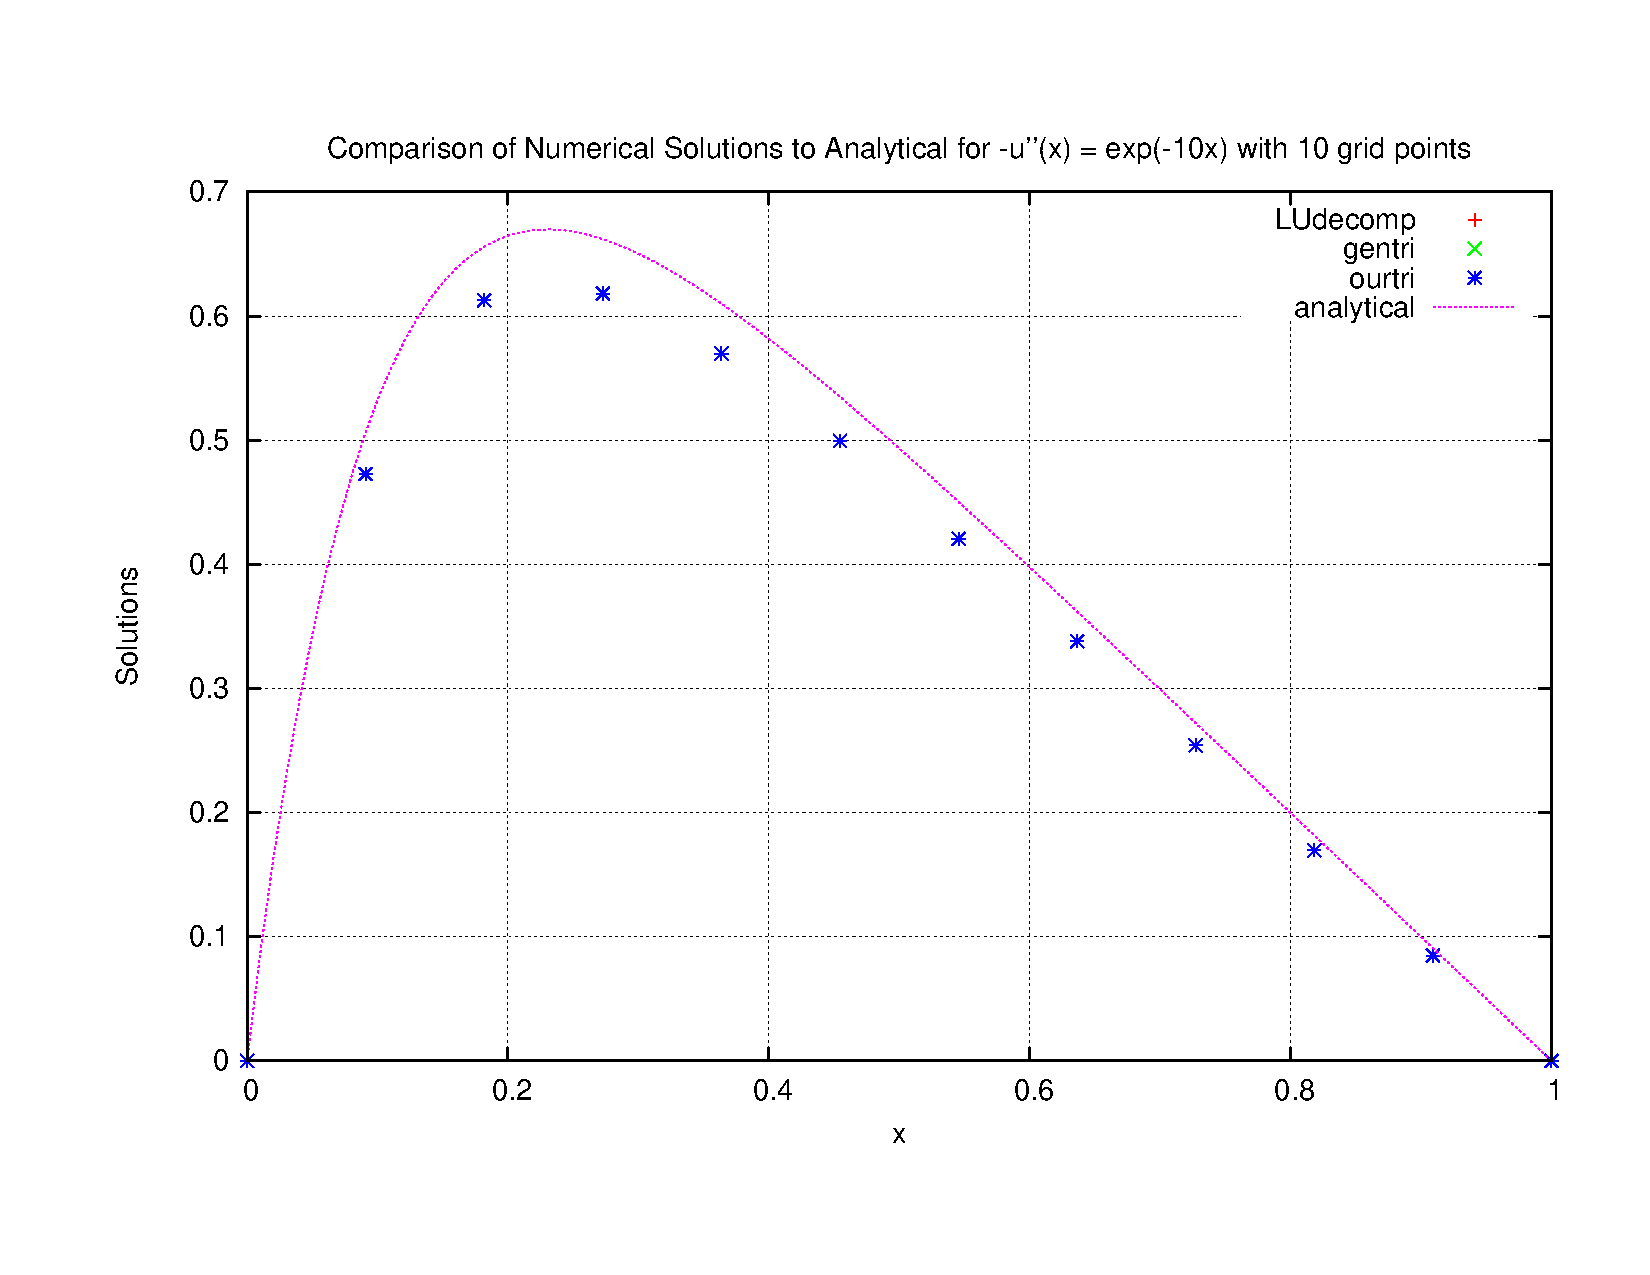
\includegraphics[width=1.0\textwidth]{comparisonplot_10.pdf}
\caption{We plot the results for $\hat{v}$ from each methodology using n=10. Note that each is nearly indistinguishable from each other; they are in fact the same to several decimal places despite all being too low.}
\end{figure}
\begin{figure}
\centering
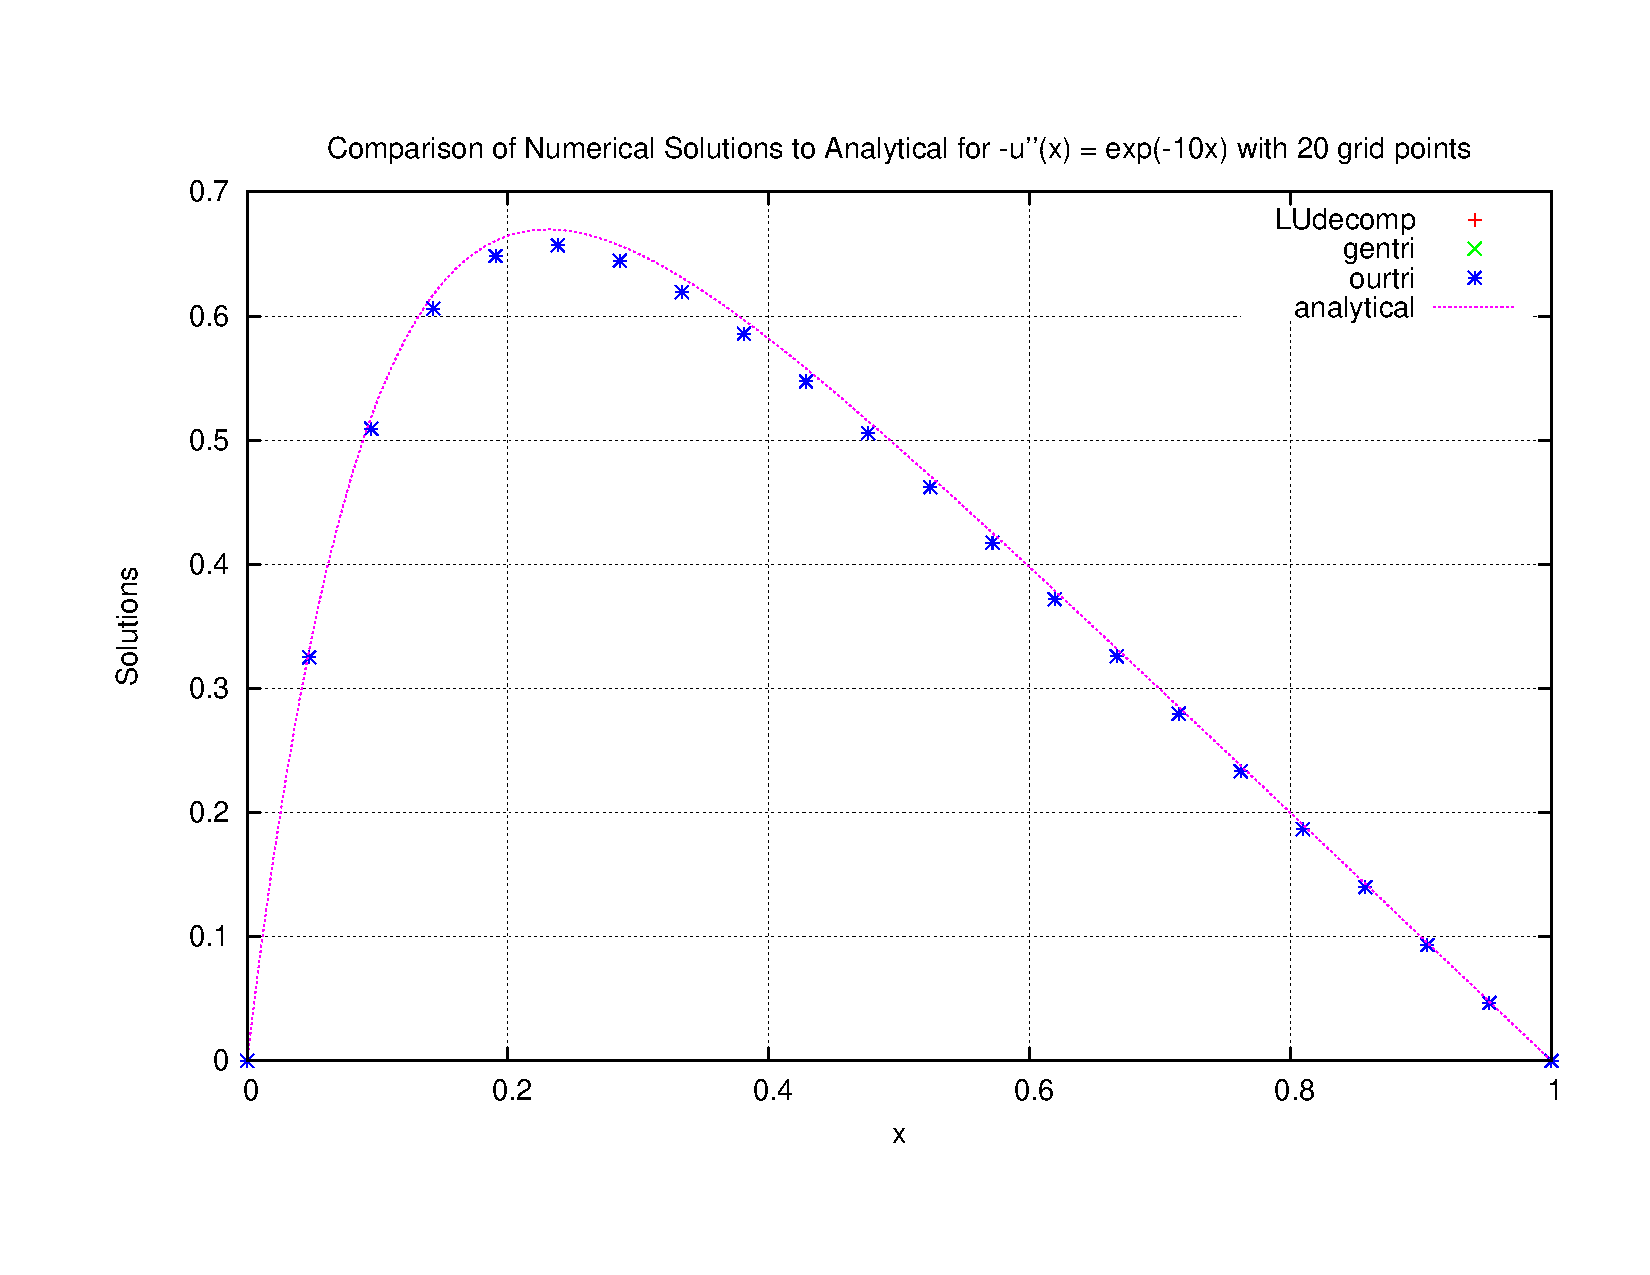
\includegraphics[width=1.0\textwidth]{comparisonplot_20.pdf}
\caption{We plot the results for $\hat{v}$ from each methodology using n=20. Obersve how even at this low count for the number of grid points, we are quickly converging to the analytical solution. Note that each is nearly indistinguishable from each other; they are in fact the same to several decimal places despite all being too low.}
\end{figure}
\begin{figure}
\centering
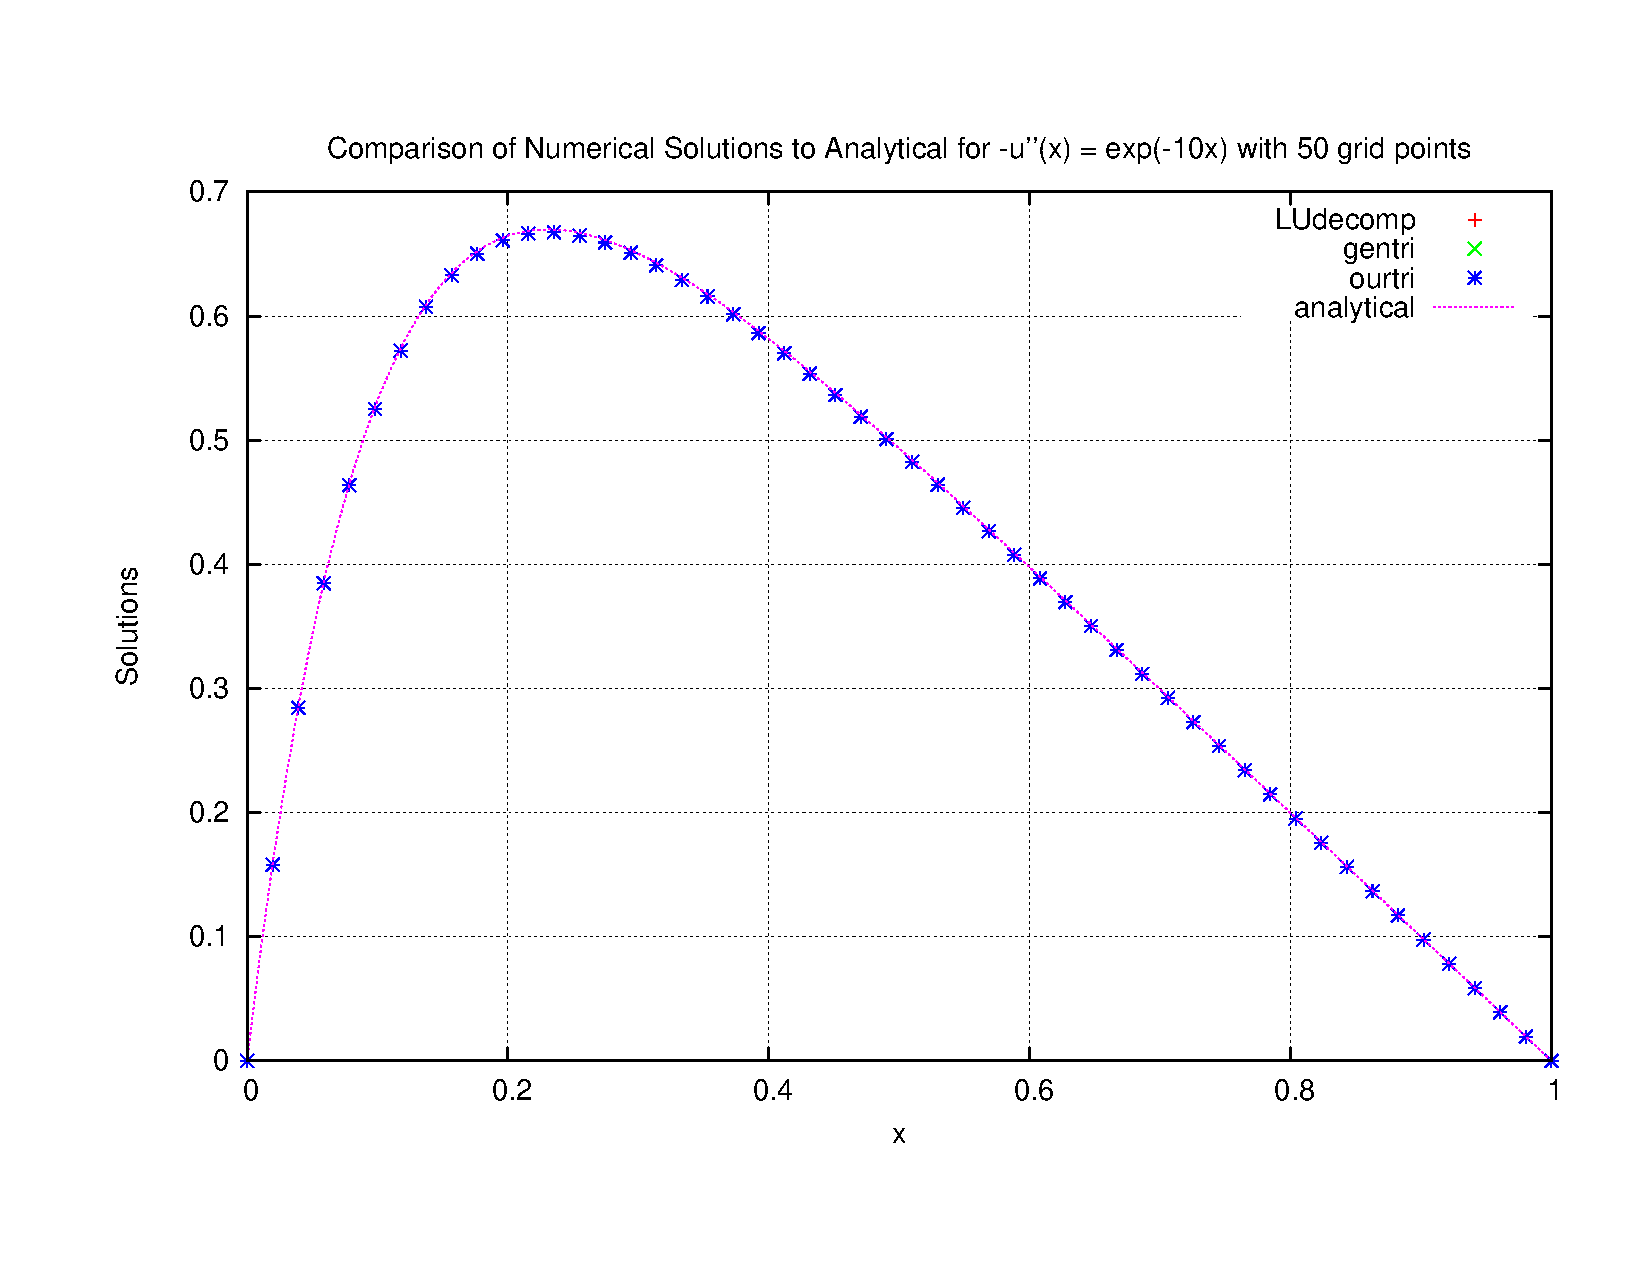
\includegraphics[width=1.0\textwidth]{comparisonplot_50.pdf}
\caption{We plot the results for $\hat{v}$ from each methodology using n=50. Now only the highest points are distinguishable from the exact solutions. Note that each is nearly indistinguishable from each other.}
\end{figure}
\begin{figure}
\centering
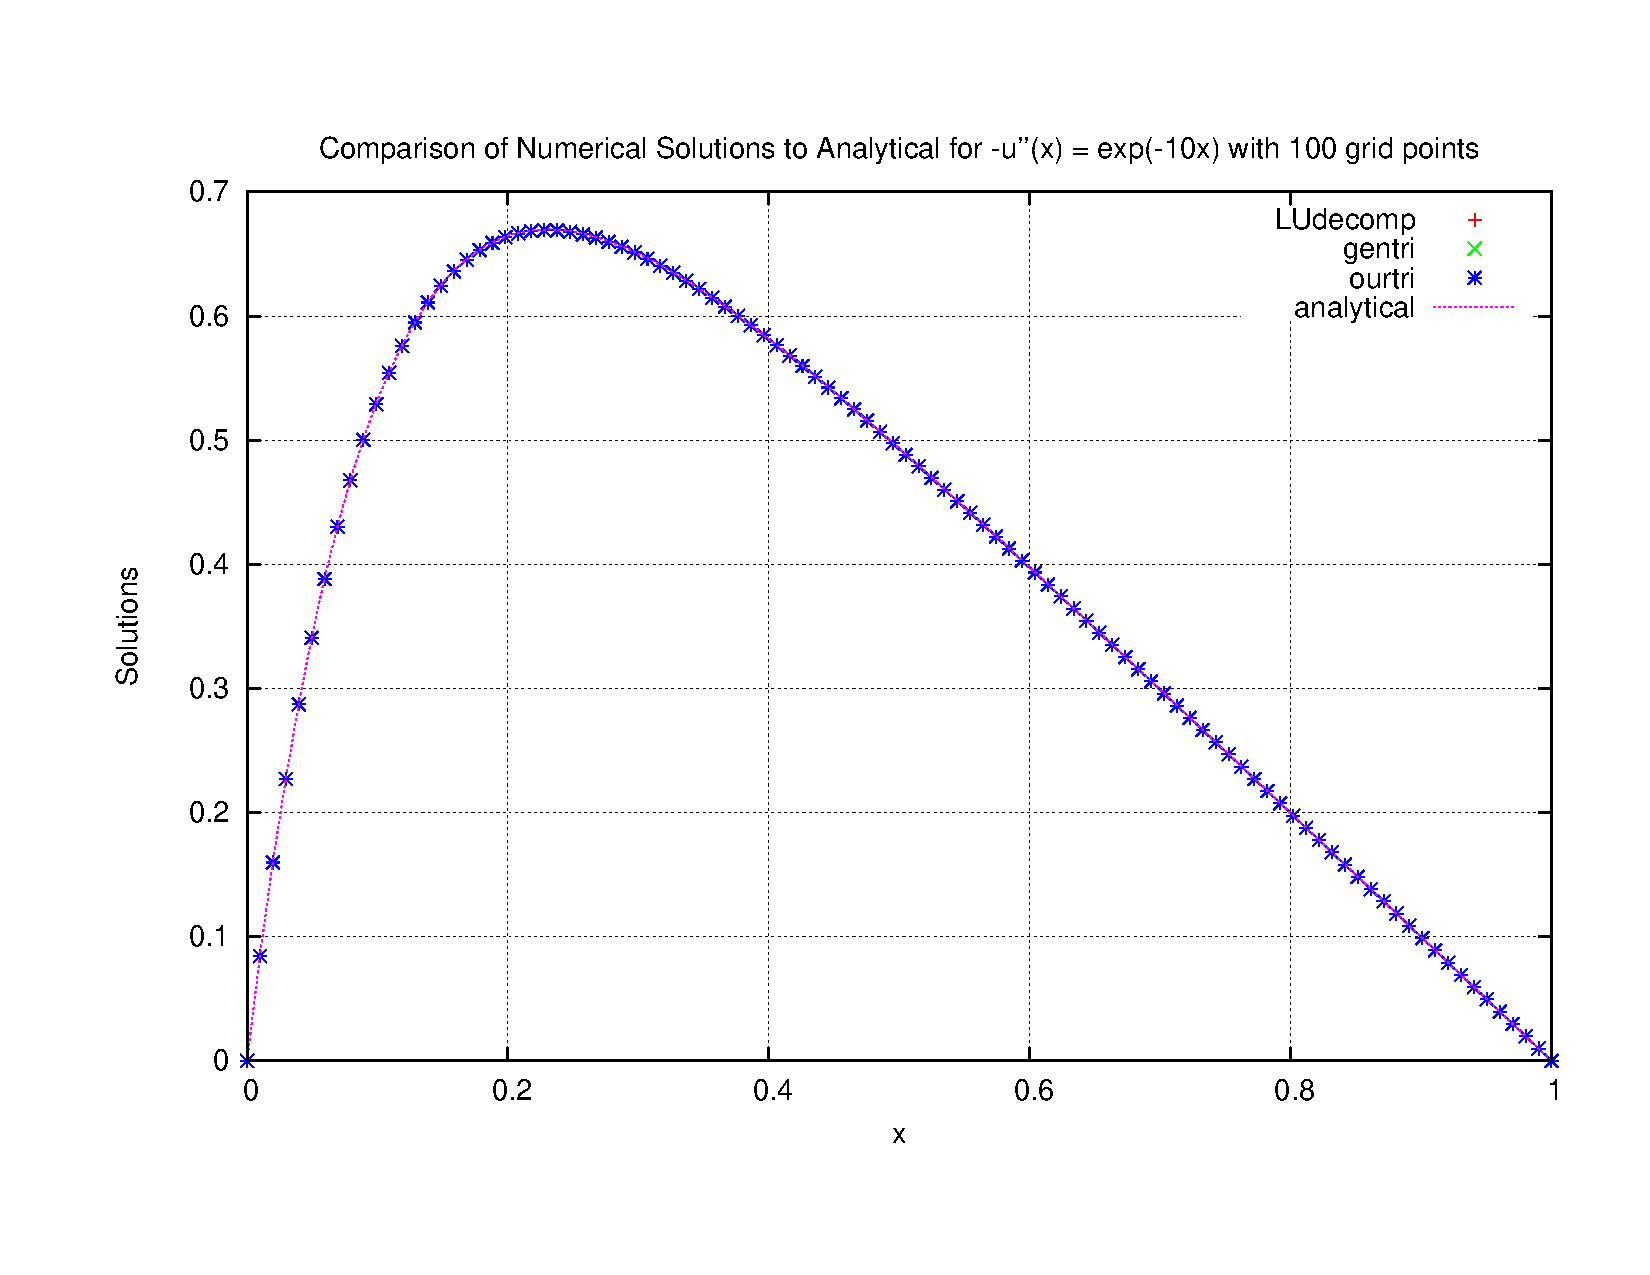
\includegraphics[width=1.0\textwidth]{comparisonplot_100.pdf}
\caption{We plot the results for $\hat{v}$ from each methodology using n=100. The numeric solutions now agree with the analytical comparison to several decimal places. Note that each is nearly indistinguishable from each other.}
\end{figure}
\begin{figure}
\centering
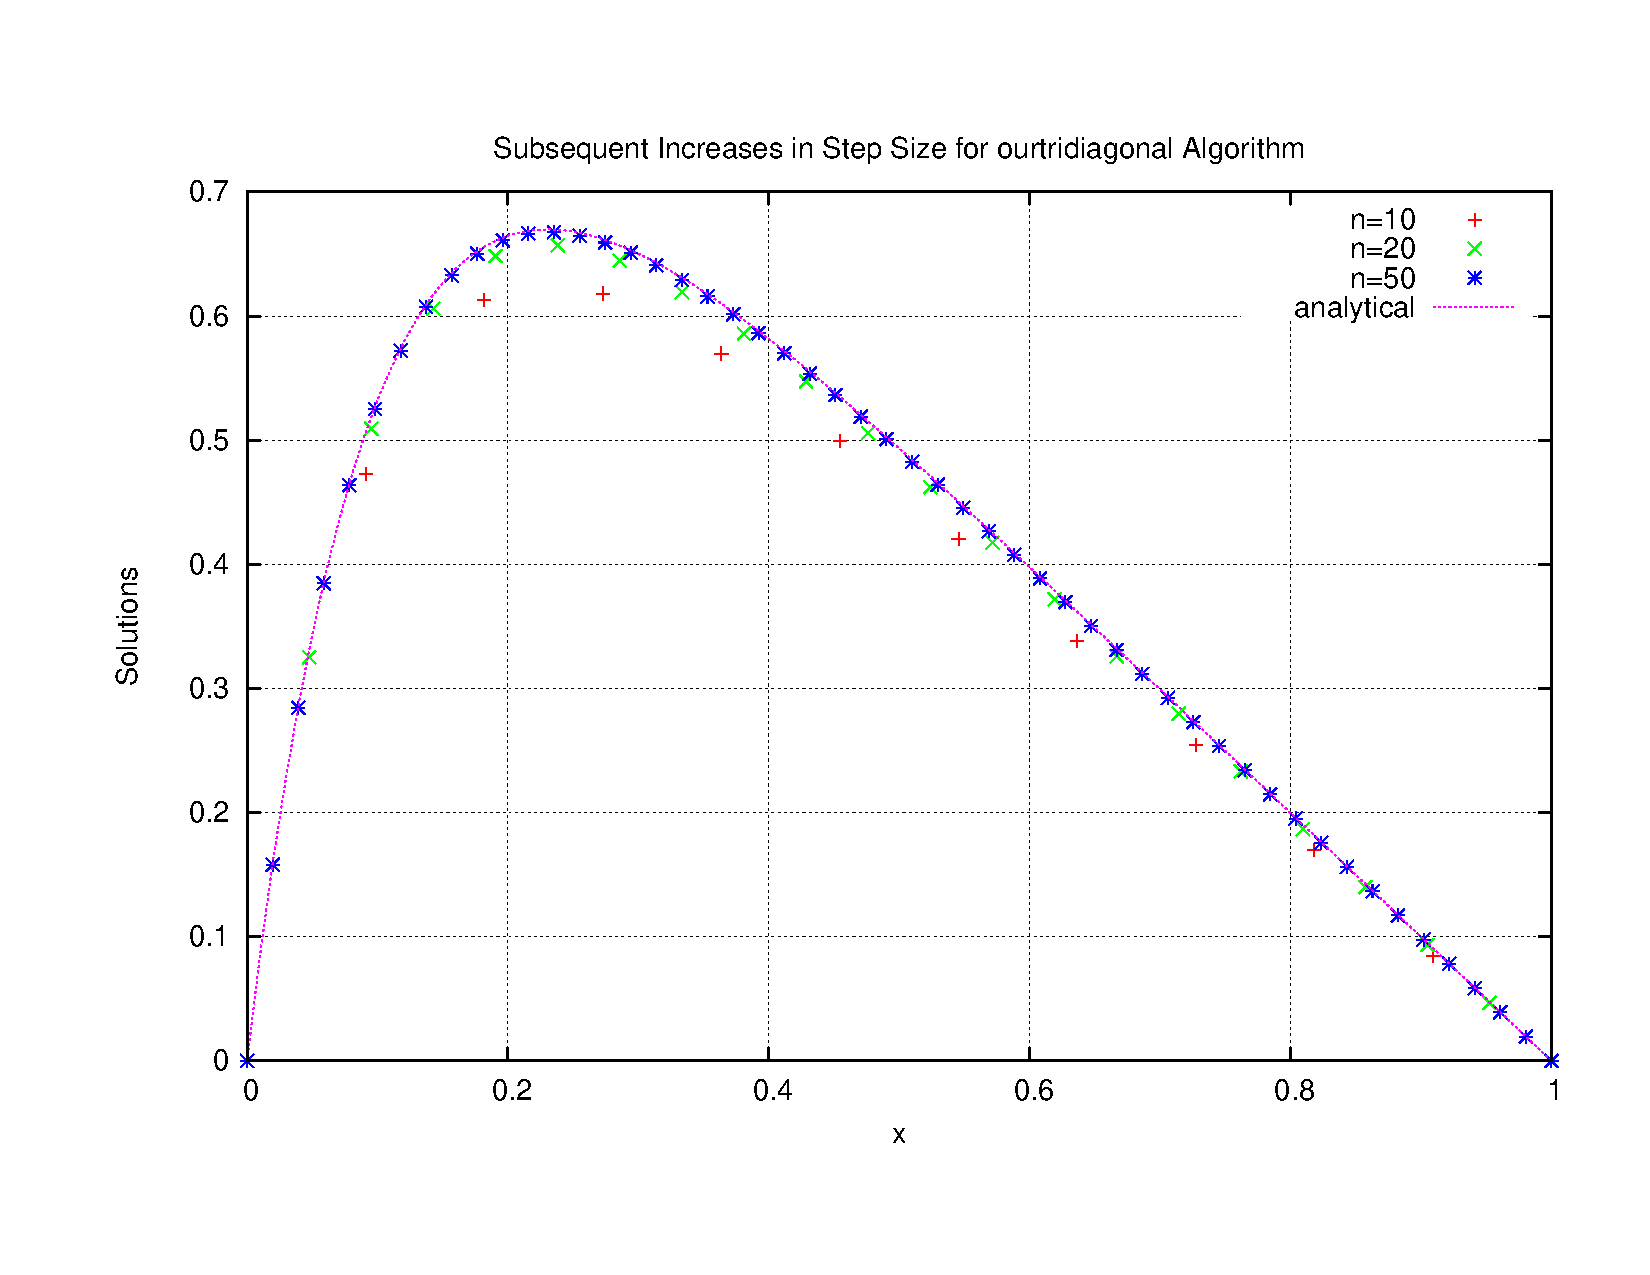
\includegraphics[width=1.0\textwidth]{comparisonourtri.pdf}
\caption{We plot the results for $\hat{v}$ from the specific tridiagonal solver using n=10, 20, and 50 to demonstrate the convergence. The specific tridiagonal was selected since it is the fastest and most stable algorithm, while also printing identical (to several decimal places) results to the others.}
\end{figure}
\begin{figure}
\centering
\begin{tabular}{| l | l | l | l |}
\hline
n & LU decomp [s] & Gen TriD [s] & Spec TriD [s] \\ \hline
5 & 2e-06 & 1e-06 & 1e-06 \\ \hline
10 & 4e-06 & 1e-06 & 1e-06 \\ \hline
50 & 0.000211 & 1e-06 & 2e-06 \\ \hline
100 & 0.001354 & 3e-06 & 2e-06 \\ \hline
500 & 0.162938 & 1.4e-05 & 1.1e-05 \\ \hline
1000 & 1.59003 & 2.9e-05 & 3.9e-05 \\ \hline
5000 & 629.842 & 0.000155 & 0.000121 \\ \hline
$10^4$ & -- & 0.00031 & 0.00018 \\ \hline
5$\times10^4$ & -- & 0.001282 & 0.000908 \\ \hline 
$10^5$ & -- & 0.003063 & 0.002118 \\ \hline
5$\times10^5$ & -- & 0.012167 & 0.009076 \\ \hline
$10^6$ & -- & 0.023728 & 0.018688 \\ \hline
5$\times10^6$ & -- & 0.123043 & 0.090099 \\ \hline
$10^7$ & -- & 0.248226 & 0.18488 \\ \hline
5$\times10^7$ & -- & 1.22033 & 0.907956 \\ \hline
\end{tabular}
\caption{A table comparing the computation times of the three algorithms for various n. Note that as n increases, LU decomposition becomes mired in computation and quickly runs for lengthy periods of time, whereas both tridiagonal solvers only pass one second computation times for n=$10^7$, before which point they've already lost stability (see Figure (7)). The general tridiagonal solver's time is typically only one-third again as large as the specific tridiagonal. This is likely because the computations it performs beyond those from the specific algorithm are not nearly as intensive as those which overlap, multiplying or dividing by (-1), for example, when including the $a_i$ and $c_i$ values.}
\end{figure}   
\begin{figure}
\centering
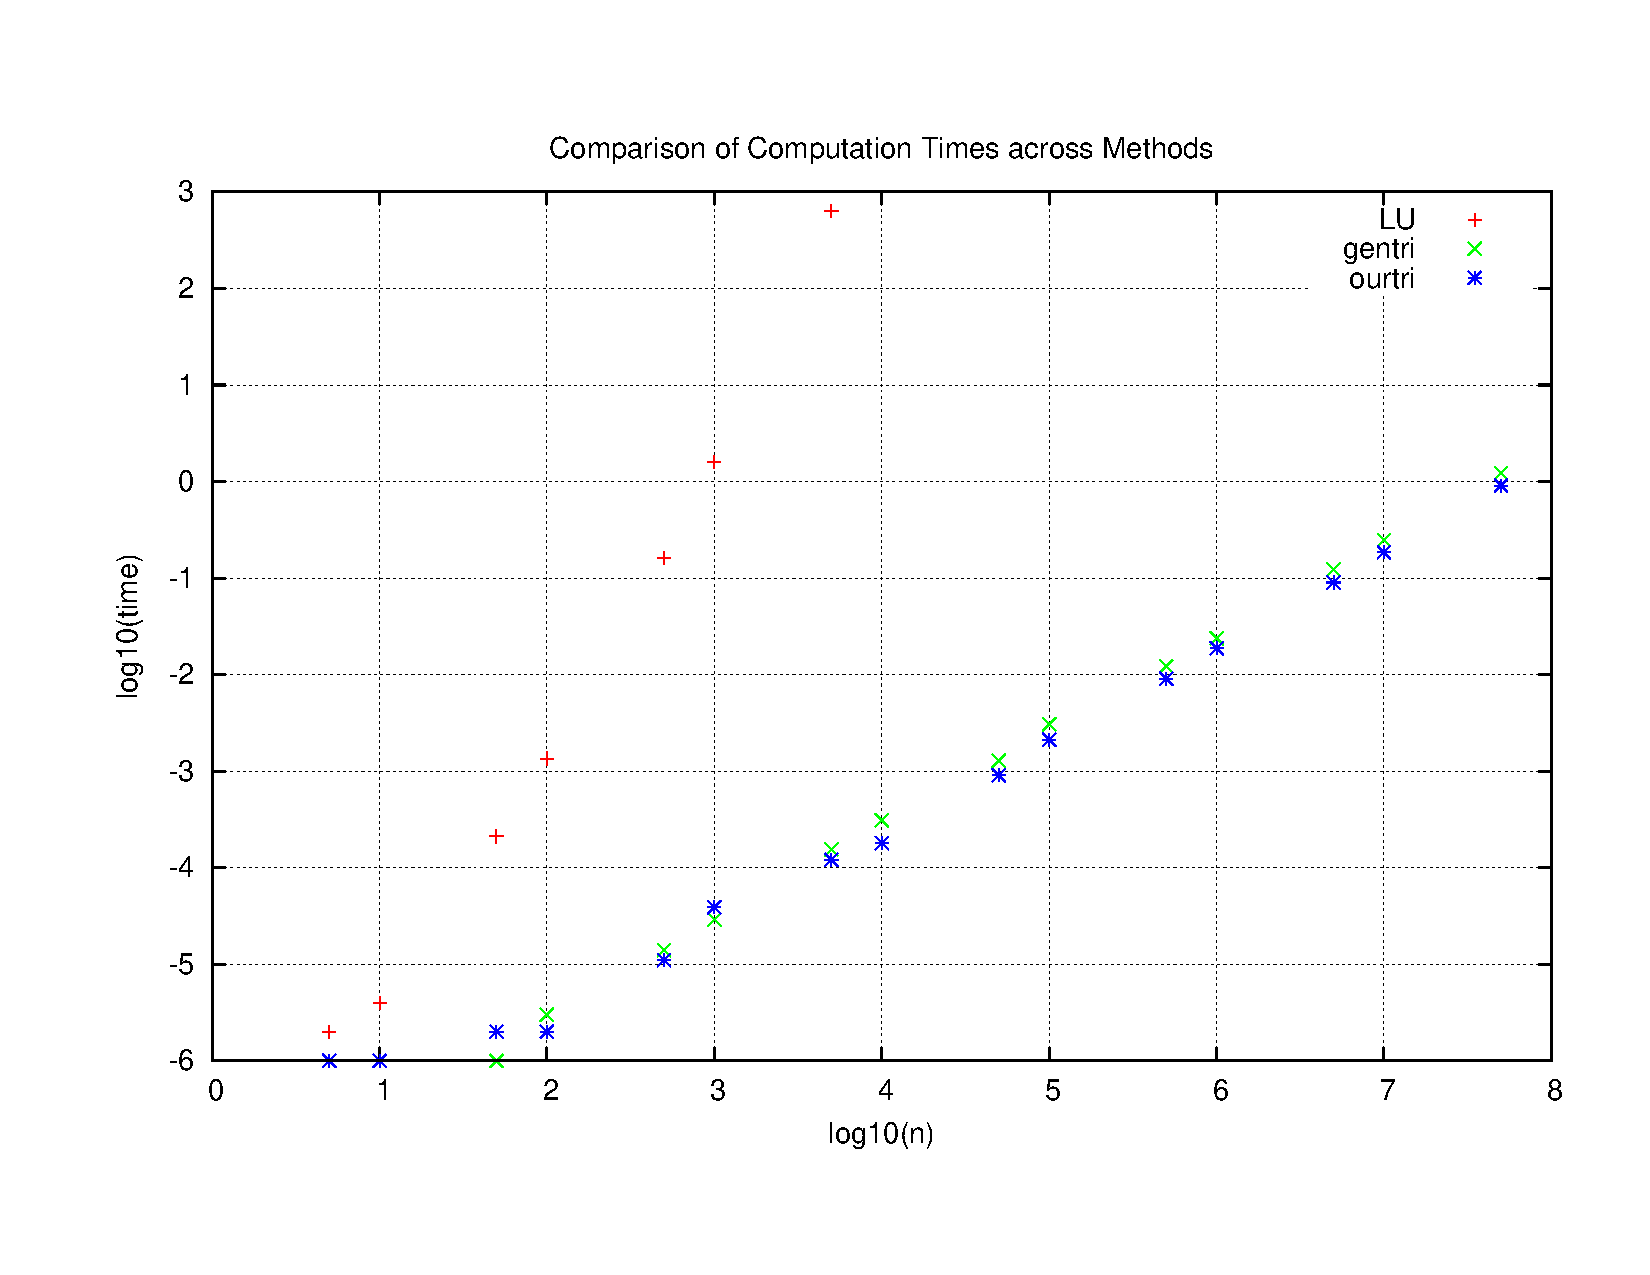
\includegraphics[width=1.0\textwidth]{comparisontime.pdf}
\caption{A plot of $log_{10}(time)$ versus $log_{10}(n)$ to demonstrate how computation time scales with the choice of n. Note that the slope for LU decomposition can be seen to be approximately three, indicating good agreement with our predicting scaling of a factor times $n^3$. Similarly, the slopes for both tridiagonal solvers are about one, in agreement with our prediction of a factor times $n^1$ for each. It is clear that both tridiagonal solvers are significantly faster than LU decomposition, with our specific solver being the fastest overall.}
\end{figure}
\begin{figure}
\centering
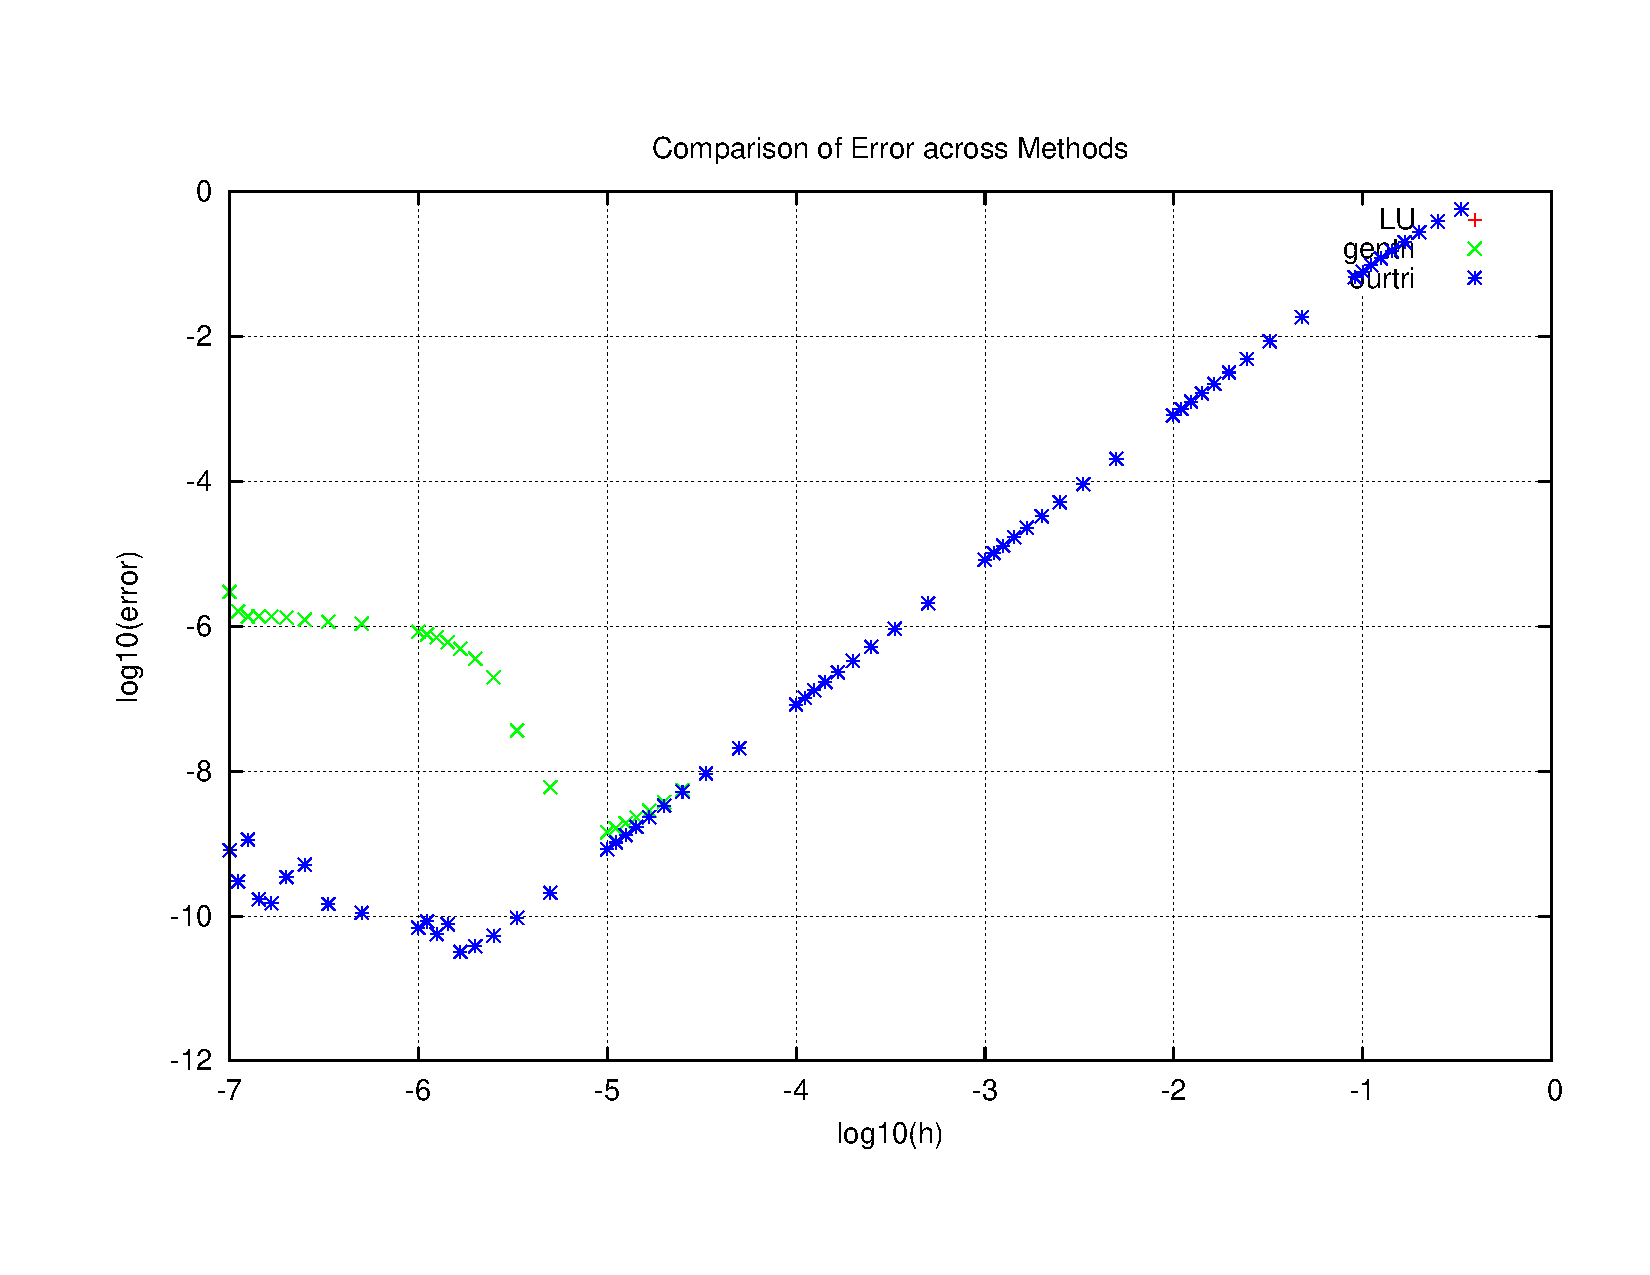
\includegraphics[width=1.0\textwidth]{comparisonerror.pdf}
\caption{A plot of $log_{10}(errors)$ versus $log_{10}(h)$. Note that for large h, or small n, the errors are nearly identical and scale as $h^2$, as we'd expect from our common approximation for the second derivative. The discrepancies arise when the accumulation of round off errors causes the function to lose stability. The specific tridiagonal solver loses stability the latest, post $10^5$ grid points. The general solver, as a result of performing more calculations, loses stability sooner, between n = $10^4$ and n = $10^5$. I was unable to run LU decomp for large enough n to find where it loses stability, but from the trend it would likely be sooner than either tridiagonal method due to the larger number of computations.}
\end{figure}

\section{Discussion}

Each aglorithm produces very similar accuracy, so discussion will focus around computation time and stability.

A brute force approach to the problem with LU decomposition results in acceptable accuracy but an extremely slow program. With times breaching one second at only 1000 grid points, LU decomposition lags significantly behind both tridiagonal solvers which only reach one second times far past where they've already lost stability. An increase by a factor of 10 in n results in a $10^3$ increase in computation time, so n=10,000 would results in computation times exceeding twenty minutes. It is the slowest algorithm and likely to lose stability first.

The general tridiagonal solver produces acceptable accuracy with fast computation times. Computation time reaches a mere 3.1$\times10^{-4}$ seconds before it approaches the region where it loses stability, post $10^4$ grid points. Computation time scales predictably with an increase of one order of magnitude for a like increase in n. The general tridiagonal solver falls solidly in the middle, with the second best stability and computation time.

The algorithm tailored for our specific chocie of approximation for the second derivative has both acceptable accuracy and the fastest computation time, as one would expect for a tailored solution. Its computation time scales as does the general solver, where an increase of one order of magnitude in n produces a like increase in computation time. It is notable that the computation time is not half that of the general solver as theory might suggest; however, this is to be expected since floating point operations are not all equal in terms of computation time. Specifically, two of the operations repeatedly performed in the general case not performed in the specific case are merely multiplication or division by (-1), a speedy process compared with division by any $b_i$. The specific solver also keeps stability for the longest, until past n=$10^5$.

The form selected for the approximation of the second derivative results in error scaling as $h^2$ in all cases, until an accumulation of round off errors results in a loss of stability.

\section{Conclusion}

In this project we have investigated three separate algorithms for solving a second order differential equation, namely LU decomposition, a general tridiagonal matrix solver, and a tridiagonal solver tailored to our specific choice for second derivative approximation. Successively, they run from the least time efficient and least stable to the most time efficient and stable. LU decomposition is by far the slowest with computation times scaling as $n^3$, whereas the tridiagonal solvers scales as $n^1$. Until each algorithm's respective loss of stability, their error scales identically with differences appearing only several decimals into each point. It is clear that the tridiagonal solver tailored to this case is the fastest and keeps stability the longest, while producing near identical results. 

\section{References}

[1] M. Hjorth-Jensen. Computational Physics, lecture notes spring 2016. Department of Physics, Michigan State University, 2016.

\newpage

\section*{Code Attachment}

\begin{lstlisting}[title={LUdecomp.cpp}]
/***************************************************************
Note that LU decomp is not possible for all matrices.
This file is designed to solve a second order differential
equation using LU decomposition of matrices. Given -u"(x) = f(x),
u(1)=u(0)=0, we approximate -u"(x) = -(v_i+1 + v_i-1 - 2*v_i)/h^2,
and solve A*v=f, where A is a tridiagonal matrix, v is our 
numerical solution, and f is our f(x) evaluated at each x_i. Each 
has dimensionality n, where n is our number of grid points. We 
define h, our step size, as 1/(n+1) so as not to include the end 
points, which we fix by definition.
****************************************************************/

#include<iostream>
#include<cmath>
#include<iomanip>
#include<fstream>
#include "time.h"

using namespace std;

ofstream ofile;

void Array_alloc(double*& a, int length);
void Matrix_alloc(double**& a, int rows, int columns);
void Array_dealloc(double*& a);
void Matrix_dealloc(double**& a, int rows);
void Matrix_LUdecomp(int size, double**& a, double**& l, double**& u);
void Matrix_Lyf_solve(int size, double**& l, double*& y, double*& func);
void Matrix_Uvy_solve(int size, double**& u, double*& v, double*& y);
void Matrix_LUdecomp_solve_complete(int size, double**& a, double*& v, double*& func);

int main(int argc, char* argv[]){
	int i, j, k, n, size, timer_data_nofile, error_yesno;
	int sizefile = 0, sizeerror=0;
	double h, time;
	double* v_lu, *y, *func;
	double** a, **u, **l;
	char* outfilename;
	clock_t start, finish;
//Desired matrix size--output file name--'1' or '0' for error file--'2', '1', '0' for timefile, numerical, or no data file, respectively
	if(argc<5){
		cout << "Bad usage. Enter also matrix_size outfilename error_yesno ('1' or '0') timer_data_nofile on same ('2','1', or '0') line." << endl;
		exit(1);
	}
	else{
		size = atoi(argv[1]);
		outfilename = argv[2];
		error_yesno = atoi(argv[3]);
		timer_data_nofile = atoi(argv[4]);
		if(timer_data_nofile==2||timer_data_nofile==1){
			ofile.open(outfilename);
		}
	}

/***************************************************************
Here the process of filtering the input data occurs.
If timer_data_nofile = 2, we created the appropriate limits for
the time file, more information below. If timer_data_nofile = 1, 
we set the forloop for one pass and merely set n to the desired 
size. If timer_data_nofile equals 0, we forgo file creation 
altogether for the loop. If error_yesno = 1, we set the 
appropriate size for sizeerror for the error loop. If error_yesno
equals 0, we forgo sizing sizeerror altogether since the loop 
will not be executed.
****************************************************************/
	
	if(timer_data_nofile==2){
		do{
			sizefile++;
			j = size/pow(10.0,sizefile);
		} while(j>1);
		if(j==1) sizefile*=2;
		if(j==0) sizefile = 2*sizefile - 1;
	}
	else if(timer_data_nofile==1){
		n=size;
		sizefile=1;
	}
	else if(timer_data_nofile==0){
		sizefile=0;
	}
	if(error_yesno==1){
		do{
			sizeerror++;
			j=size/pow(10.0,sizeerror);
		} while (j>1);
	}
		
/***************************************************************
Note the structure presented here. If a time file is called for, 
we perform the loops at n = 5, 10, 50, 100, 500, 100, etc until 
the first number in this series greater than or equal to the 
desired matrix size, writing each respective n and time to the
entered outfilename. If a numerical data file is called for, we
simply perform one loop and output the data itself. If no file
is called, the loop does not execute.
****************************************************************/
	
	for(k=1;k<=sizefile;k++){
		if(timer_data_nofile==2){
			if(k%2==0) n=pow(10.0,k/2);
			else n=pow(10.0,(k+1)/2)/2;
		}
	
		h=(1.0/(double) (n+1));
	
//Allocate the arrays and matrices

		Array_alloc(v_lu, n); Array_alloc(y, n); Array_alloc(func, n);
		Matrix_alloc(a, n, n); Matrix_alloc(u, n, n); Matrix_alloc(l, n, n);

//Initialize func[i] values && a[i][j]

		for(i=0;i<n;i++){
			func[i]=pow(h, 2.0)*100.0*exp(-10.0*h*((double) (i+1)));
		}
		for(i=0;i<n;i++){
			for(j=0;j<n;j++){
				if(i==j) a[i][j]=2.0;
				else if((i+1)==j||(i-1)==j) a[i][j]=-1.0;
				else a[i][j]=0.0;
			}
		}

/*********************
Begin computation time
**********************/

		start = clock();

//Here we conduct the decomp

		Matrix_LUdecomp(n, a, l, u);

//Calculate y from L*y=func	

		Matrix_Lyf_solve(n, l, y, func);

//Calculcate v_lu from U*v_lu=y

		Matrix_Uvy_solve(n, u, v_lu, y);

		finish = clock();

/*******************
End computation time
********************/

		time = ((finish-start)/(double) CLOCKS_PER_SEC);

		if(timer_data_nofile==1) cout << '\t' << time << " seconds" << endl;

//Write to file

		if(timer_data_nofile==2){
			ofile.precision(6);
			if(k==1) ofile << "#_n" << setw(15) << "log10(n)" << setw(15) << "time" << setw(15) << "log10(time)" << endl;
			ofile << n << setw(15) << log10(n) << setw(15) << time << setw(15) << log10(time) << endl;
		}		
		else if(timer_data_nofile==1){
			for(i=0;i<n;i++){
				ofile << h*(double) (i+1) << setw(20) << v_lu[i] << endl;
			}
		}
		
		Array_dealloc(y); Array_dealloc(v_lu); Array_dealloc(func);
		Matrix_dealloc(a,n); Matrix_dealloc(u,n); Matrix_dealloc(l,n);
	}
	
	if(timer_data_nofile==2||timer_data_nofile==1){
		ofile.close();
	}

/***************************************************************
Calculate error if desired, up to file size provided by input.
Note that it outputs maximum error for 2,3,4,...,9,10,20,30...,
90,100,200,... up to the 10^(ceiling(power of ten of input)),
minimum of 10^1.
****************************************************************/


	if(error_yesno==1){
		ofile.open("LUerror.dat");
		ofile.precision(8);
		ofile << "#_n" << setw(15) << "log(h)" << setw(20) << "max_log(error)" << endl;
		double exact, x, temp, error;
		int m;
		for(m=0;m<sizeerror;m++){
			for(k=2;k<=10;k++){
				n=k*pow(10,m);
				h=(1.0/(double) (n+1));
				Array_alloc(v_lu, n); Array_alloc(func, n);
				Matrix_alloc(a, n, n);
				
				for(i=0;i<n;i++){
					func[i]=pow(h, 2.0)*100.0*exp(-10.0*h*((double) (i+1)));
				}
				for(i=0;i<n;i++){
					for(j=0;j<n;j++){
						if(i==j) a[i][j]=2.0;
						else if((i+1)==j||(i-1)==j) a[i][j]=-1.0;
						else a[i][j]=0.0;
					}
				}

				Matrix_LUdecomp_solve_complete(n, a, v_lu, func);

				error=-20.0;
				for(i=0;i<n;i++){
					temp = 0.0;
					x = (i+1)*h;
					exact = 1.0 - (1.0 - exp(-10.0))*x-exp(-10.0*x);
					temp = log10(abs(v_lu[i]-exact)/exact);
					if(temp>error) error = temp;
				}

				ofile << n << setw(20-m) << log10(h) << setw(15) << error << endl;

				Array_dealloc(v_lu); Array_dealloc(func);
				Matrix_dealloc(a, n);
			}
		}
	}


	return 0;
}




/**************************
Begin function definitions
***************************/

void Array_alloc(double*& a, int length){
	a = new double[length];
}

void Matrix_alloc(double**& a, int rows, int columns){
	a = new double* [rows];
	for(int count=0;count<rows;count++){
		a[count] = new double [columns];
	}
}

void Array_dealloc(double*& a){
	delete[] a;
}

void Matrix_dealloc(double**& a, int rows){
	for(int i=0;i<rows;i++){
		delete[] a[i];
	}
	delete[] a;
}

void Matrix_LUdecomp(int size, double**& a, double**& l, double**& u){
	int i, j, k;	
	for(i=0; i<size;i++){
		for(j=0;j<size;j++){
			l[i][j]=0.0;
			u[i][j]=0.0;
		}
		l[i][i]=1.0;
	}
	for(i=0; i<size;i++){
		double temp;
		for(j=i;j<size;j++){
			temp = 0.0;
			for(k=0;k<i;k++){
				temp +=l[i][k]*u[k][j];
			}
			u[i][j] = a[i][j] - temp;
		}
		for(j=i+1;j<size;j++){
			temp = 0.0;
			for(k=0;k<i;k++){
				temp +=l[j][k]*u[k][i];
			}
			 l[j][i] = (a[j][i] - temp)/u[i][i];
		}
	}
}

void Matrix_Lyf_solve(int size, double**& l, double*& y, double*& func){
	int i, j;	
	for(i=0;i<size;i++){
		double temp = 0.0;
		for(j=0;j<i;j++){
			temp += l[i][j]*y[j];
		}
		y[i]=func[i]-temp;
	}
}

void Matrix_Uvy_solve(int size, double**& u, double*& v, double*& y){
	int i, j;	
	for(i=size-1;i>=0;i--){
		double temp = 0.0;
		for(j=i+1;j<size;j++){
			temp += u[i][j]*v[j];
		}
		v[i] = (y[i]-temp)/u[i][i];
	}
}

void Matrix_LUdecomp_solve_complete(int size, double**& a, double*& v, double*& func){
	int i, j, k;
	double** l, **u;
	double* y;
	l = new double* [size];
	for(int i=0;i<size;i++){
		l[i] = new double [size];
	}	
	u = new double* [size];
	for(int i=0;i<size;i++){
		u[i] = new double [size];
	}
	y = new double[size];

	for(i=0; i<size;i++){
		for(j=0;j<size;j++){
			l[i][j]=0.0;
			u[i][j]=0.0;
		}
		l[i][i]=1.0;
	}

	for(i=0; i<size;i++){
		double temp;
		for(j=i;j<size;j++){
			temp = 0.0;
			for(k=0;k<i;k++){
				temp +=l[i][k]*u[k][j];
			}
			u[i][j] = a[i][j] - temp;
		}
		for(j=i+1;j<size;j++){
			temp = 0.0;
			for(k=0;k<i;k++){
				temp +=l[j][k]*u[k][i];
			}
			 l[j][i] = (a[j][i] - temp)/u[i][i];
		}
	}

	for(i=0;i<size;i++){
		double temp = 0.0;
		for(j=0;j<i;j++){
			temp += l[i][j]*y[j];
		}
		y[i]=func[i]-temp;
	}
	for(i=size-1;i>=0;i--){
		double temp = 0.0;
		for(j=i+1;j<size;j++){
			temp += u[i][j]*v[j];
		}
		v[i] = (y[i]-temp)/u[i][i];
	}

	for(int i=0;i<size;i++){
		delete[] l[i];
		delete[] u[i];
	}
	delete[] l;
	delete[] u;
	delete[] y;
}
\end{lstlisting}

\begin{lstlisting}[title={tridiag.cpp}]
/***************************************************************
This file is designed to solve a second order differential
equation by discretizing the domain into x_i's and forming a 
linear algebra problem. Given -u"(x) = f(x), u(1)=u(0)=0, we 
approximate -u"(x_i) = -(v_i+1 + v_i-1 - 2*v_i)/h^2 = f(x_i), and 
solve A*v=f, where A is a tridiagonal matrix, v is an array of 
our numerical solution, and f is an array of our f(x_i). Each has 
dimensionality n, where n is our number of grid points. We 
define h, our step size, as 1/(n+1) so as not to include the end 
points, which we fix by definition.

Here we simplify the problem due to A's tridiagonal form, first
solving for a general tridiagonal matrix, then recognizing the 
inherent symmetry to reduce the number of floating points 
operatings required by half. We speed the process by allocating 
space for only three arrays to represent the diagonal and 
off-diagonal elements, as shown below. 

A = ( b_1 c_1  0   0   0  ...  0   0  )
    ( a_2 b_2 c_2  0   0  ...  0   0  )
    (  0  a_3 b_3 c_3  0  ...  0   0  )
    ( ... ... ... ... ... ... ... ... )
    (  0   0   0   0  ...  0  a_n b_n )

****************************************************************/

#include<iostream>
#include<cmath>
#include<iomanip>
#include<fstream>
#include "time.h"

using namespace std;

ofstream ofile;

void Array_alloc(double*& a, int length);
void Matrix_alloc(double**& a, int rows, int columns);
void Array_dealloc(double*& a);
void Matrix_dealloc(double**& a, int rows);
void gen_tridmat_equ_solve(int n, double*& a, double*& b, double*& c, double*& v, double*& func);
void secder_tridmat_equ_solve(int n, double*& b, double*& v, double*& func);

int main(int argc, char* argv[]){
	char* outfilename;
	int n, i, j, k, error_yesno, timer_data_nofile, size;
	int sizefile = 0, sizeerror=0;
	double h, time1, time2;
	double* a, *b, *c, *v1, *v2, *func;
	clock_t start, finish;

	if(argc<5){
		cout << "Bad usage. Enter also grid_point_count outfilename error_yesno ('1' or '0') timer_data_nofile on same ('2','1', or '0') line." << endl;
		exit (1);
	}
	else{
		size = atoi(argv[1]);
		outfilename = argv[2];
		error_yesno = atoi(argv[3]);
		timer_data_nofile = atoi(argv[4]);
		if(timer_data_nofile==2||timer_data_nofile==1){
			ofile.open(outfilename);
		}
	}

/***************************************************************
Here the process of filtering the input data occurs.
If timer_data_nofile = 2, we created the appropriate limits for
the time file, more information below. If timer_data_nofile = 1, 
we set the forloop for one pass and merely set n to the desired 
size. If timer_data_nofile equals 0, we forgo file creation 
altogether for the loop. If error_yesno = 1, we set the 
appropriate size for sizeerror for the error loop. If error_yesno
equals 0, we forgo sizing sizeerror altogether since the loop 
will not be executed.
****************************************************************/
	
	if(timer_data_nofile==2){
		do{
			sizefile++;
			j = size/pow(10.0,sizefile);
		} while(j>1);
		if(j==1) sizefile*=2;
		if(j==0) sizefile = 2*sizefile - 1;
	}
	else if(timer_data_nofile==1){
		n=size;
		sizefile=1;
	}
	else if(timer_data_nofile==0){
		sizefile=0;
	}
	if(error_yesno==1){
		do{
			sizeerror++;
			j=size/pow(10.0,sizeerror);
		} while (j>1);
	}

/***************************************************************
Note the structure presented here. If a time file is called for, 
we perform the loops at n = 5, 10, 50, 100, 500, 100, etc until 
the first number in this series greater than or equal to the 
desired matrix size, writing each respective n and time to the
entered outfilename. If a numerical data file is called for, we
simply perform one loop and output the data itself.
****************************************************************/

	for(k=1;k<=sizefile;k++){
		if(timer_data_nofile==2){
			if(k%2==0) n=pow(10.0,k/2);
			else n=pow(10.0,(k+1)/2)/2;
		}
	
		h=(1.0/(double) (n+1));

//Dynamically allocate memory
	
		Array_alloc(a,n); Array_alloc(b,n); Array_alloc(c,n); Array_alloc(v1,n); Array_alloc(v2,n); Array_alloc(func, n);

//Initialize array values

		for(i=0;i<n;i++){
			a[i]=(-1.0);
			b[i]=(2.0);
			c[i]=(-1.0);
			func[i]=pow(h, 2.0)*100.0*exp(-10.0*h*((double) (i+1)));
		}

/********************************************
  Start clock for general tridiagonal matrix
  Create upper diagonal matrix
  Back substitutions
  End clock
*********************************************/

		start = clock();
	
		gen_tridmat_equ_solve(n, a, b, c, v1, func);

		finish = clock();
		time1 = ( (finish - start)/(double) CLOCKS_PER_SEC);

//redfine b values for our specific tridiagonal, reinitialize func[i] values

		for(i=0;i<n;i++){
			b[i]=(double) (i+2)/(double) (i+1);
			func[i]=pow(h, 2.0)*100.0*exp(-10.0*h*((double) (i+1)));
		}

/********************************************
  Start clock for our specific tridiagonal
  Form A into upper diagonal
  Back substitutions
  End clock
*********************************************/

		start = clock();

		secder_tridmat_equ_solve(n, b, v2, func);
	
		finish = clock();
		time2 = ((finish-start)/(double) CLOCKS_PER_SEC);

//Write data file

		if(timer_data_nofile==2){
			ofile.precision(6);
			if(k==1){
				ofile << "#_n" << setw(15) << "log10(n)" << setw(15) << "time_gen" << setw(15);
				ofile << "log10(time_gen)" << setw(15) << "time_our" << setw(15) << "log10(time_our)" << endl;	
			}						
			ofile << n << setw(15) << log10(n) << setw(15) << time1 << setw(15)<< log10(time1) << setw(15) << time2 << setw(15) << log10(time2) << endl;
		}
		else if(timer_data_nofile==1){
			ofile << "#_x_i" << setw(15) << "v1(x_i)" << setw(15) << "v2(x_i)" << setw(15) << "u(x_i)" << endl;
			ofile.precision(8);		
			ofile << "1" << setw(15) << "0" << setw(15) << "0" << endl;
			for(i=n-1;i>=0;i--){
				double exact, x;
				x = (i+1)*h;
				exact = 1.0 - (1.0 - exp(-10.0))*x-exp(-10.0*x);
				ofile << x << setw(15) << v1[i] << setw(15) << v2[i] << setw(15) << exact << endl;
			}
			ofile << "0" << setw(15) << "0" << setw(15) << "0" << endl;
		}
		
		Array_dealloc(a); Array_dealloc(b); Array_dealloc(c);
		Array_dealloc(v1); Array_dealloc(v2); Array_dealloc(func);
	}
	
	if(timer_data_nofile==2||timer_data_nofile==1){
		ofile.close();
	}

//Write time to screen if creating a data file
	
	if(timer_data_nofile==1){
		cout.precision(5);
		cout << scientific;
		cout << "\tv1: " << time1 << " seconds" << endl;
		cout << "\tv2: " << time2 << " seconds" << endl;
	}

//Compute error for varying step counts, if desired

	if(error_yesno==1){
		ofile.open("trid_error.dat");
		ofile.precision(8);
		ofile << "#_n" << setw(15) << "log(h)" << setw(20) << "max_log(error1)" << setw(15) << "max_log(error2)" << endl;
		double exact, x, temp1, temp2, error1, error2;
		int m;
		for(m=0;m<sizeerror;m++){
			for(k=2;k<=10;k++){
				n = k*pow(10,m);
				double* a, *b1, *b2, *c, *func1, *func2, *v1, *v2;
				Array_alloc(a,n); Array_alloc(b1,n); Array_alloc(b2,n); Array_alloc(c,n);
				Array_alloc(func1,n); Array_alloc(func2,n); Array_alloc(v1,n); Array_alloc(v2,n);
				
				h = 1.0/((double) (n+1));
				for(i=0;i<n;i++){
					a[i]=(-1.0);
					b1[i]=(2.0);
					c[i]=(-1.0);
					func1[i]=pow(h, 2.0)*100.0*exp(-10.0*h*((double) (i+1)));
					b2[i]=(double) (i+2)/(double) (i+1);
					func2[i]=pow(h, 2.0)*100.0*exp(-10.0*h*((double) (i+1)));
				}	

				gen_tridmat_equ_solve(n, a, b1, c, v1, func1);
				secder_tridmat_equ_solve(n, b2, v2, func2);
				
				error1=-20.0;
				error2=-20.0;
				for(i=0;i<n;i++){
					temp1 = 0.0;
					temp2 = 0.0;
					x = (double) (i+1)*h;
					exact = 1.0 - (1.0 - exp(-10.0))*x-exp(-10.0*x);
					temp1 = log10(abs(v1[i]-exact)/exact);
					temp2 = log10(abs(v2[i]-exact)/exact);
					if(temp1>error1) error1 = temp1;
					if(temp2>error2) error2 = temp2;
				}
				ofile << n << setw(20-m) << log10(h) << setw(15) << error1 << setw(15) << error2 << endl;

				Array_dealloc(a); Array_dealloc(b1); Array_dealloc(b2); Array_dealloc(c);
				Array_dealloc(func1); Array_dealloc(func2); Array_dealloc(v1); Array_dealloc(v2);
			}
		}
	}


	return 0;
}	




/**************************
Begin function definitions
***************************/

void Array_alloc(double*& a, int length){
	a = new double[length];
}

void Matrix_alloc(double**& a, int rows, int columns){
	a = new double* [rows];
	for(int count=0;count<rows;count++){
		a[count] = new double [columns];
	}
}

void Array_dealloc(double*& a){
	delete[] a;
}

void Matrix_dealloc(double**& a, int rows){
	for(int i=0;i<rows;i++){
		delete[] a[i];
	}
	delete[] a;
}

void gen_tridmat_equ_solve(int n, double*& a, double*& b, double*& c, double*& v, double*& func){
	int i;
	for(i=1;i<n;i++){
		double temp;
		temp = a[i]/b[i-1];
		b[i] -= temp*c[i-1];
		func[i] -= temp*func[i-1];
	}
	v[n-1]=func[n-1]/b[n-1];
	for(i=n-2;i>=0;i--){
		v[i] = (func[i]-c[i]*v[i+1])/b[i];
	}
}

void secder_tridmat_equ_solve(int n, double*& b, double*& v, double*& func){
	int i;	
	for(i=1;i<n;i++){
		func[i] += func[i-1]/b[i-1];
	}
	v[n-1]=func[n-1]/b[n-1];
	for(i=n-2;i>=0;i--){
		v[i] = (func[i]+v[i+1])/b[i];
	}
}

\end{lstlisting}
\end{document}


